\section{后缀数组}

\subsection{模板}
\begin{itemize}
    \item $sa[i]$:排名为 $i$ 的后缀的起始下标(排第 $i$ 的是哪个后缀)
    \item $rank[i]$:起始下标为 $i$ 的后缀 $suffix(i ... len-1)$ 的排名(第 $i$ 个后缀排第几),满足 $sa[rank[i]] = i, rank[sa[i]] = i$.
    \item $height[i]$: $sa[i]$ 与 $sa[i-1]$(排名相邻的两个后缀) 的最长公共前缀。
    \item $h[i] = height[rank[i]]$: $suffix(i)$ 和在他前一名的后缀的最长公共前缀。满足 $h[i] \ge h[i-1] - 1$.
\end{itemize}

\begin{minted}{c++}
namespace Suffix_Array {
    // sa[i]: 排名是i位的是第几个后缀
    // rk[i]: 第i个后缀的排名是多少
    // height[i]: sa[i]与sa[i-1]
    const int N=1000010;
    char s[N];
    int rk[N],sa[N],c[N],height[N];
    int x[N],y[N];
    int n,m;
    void rsort()// x[i] 第一关键字 y[i] 第二关键字 基数排序
    {
        for(int i=1;i<=m;i++) c[i]=0;
        for(int i=1;i<=n;i++) c[x[i]]++;
        for(int i=1;i<=m;i++) c[i]+=c[i-1];
        for(int i=n;i;i--) sa[c[x[y[i]]]--]=y[i];
    }
    void build_sa()
    {
        n=strlen(s+1);
        m=256;
        for(int i=1;i<=n;i++) x[i]=s[i],y[i]=i;
        rsort();
        for(int k=1;k<=n;k<<=1)
        {
            int p=0;
            for(int i=n-k+1;i<=n;i++) y[++p]=i;// 第二关键字为空字符排在最前面
            for(int i=1;i<=n;i++) if(sa[i]>k) y[++p]=sa[i]-k;
            rsort();swap(x,y);
    
            x[sa[1]]=1,p=1;
            for(int i=2;i<=n;i++)
                x[sa[i]]=(y[sa[i]]==y[sa[i-1]]&&y[sa[i]+k]==y[sa[i-1]+k]?p:++p);
            if(p==n) break;
            m=p;
        }
    }
    void get_height()
    {
        for(int i=1;i<=n;i++) rk[sa[i]]=i;
        // 求height
        for(int i=1,j=0;i<=n;i++)
        {
            if(j) --j;
            while(s[i+j]==s[sa[rk[i]-1]+j]) j++;
            height[rk[i]]=j;
        }
    }
    // 求lcp 有时需要找到本质不同第k大最早出现的位置
    // 首先二分能找到第k大,然后再次二分找到[sa[l]....sa[r]] 取最小值就是最早出现的位置
    int mnht[N][22];
    int mnsa[N][22];
    int lg[N];
    void init() {
        lg[0]=-1;
        for(int i=1;i<=n;i++) lg[i]=lg[i>>1]+1;
        for(int i=1;i<=n;i++) mnht[i][0]=height[i],mnsa[i][0]=sa[i];
        for(int j=1;j<=lg[n];j++)
            for(int i=1;i+(1<<j)-1<=n;i++)
                mnht[i][j]=min(mnht[i][j-1],mnht[i+(1<<j-1)][j-1]),\
                mnsa[i][j]=min(mnsa[i][j-1],mnsa[i+(1<<j-1)][j-1]);
    }
    int MIN(int a[][22],int l,int r)
    {
        int k=lg[r-l+1];
        return min(a[l][k],a[r-(1<<k)+1][k]);
    }
    // 询问 suffix(a) 和 suffix(b) 的最长公共前缀
    int lcp(int a,int b) 
    {
        a=rk[a],b=rk[b];
        if(a>b) swap(a,b);
        a++;
        int k=lg[b-a+1];
        return min(mnht[a][k],mnht[b-(1<<k)+1][k]);
    }
    
}using namespace Suffix_Array;
\end{minted}
\subsection{SA 应用}
\subsubsection{寻找最小的循环移动位置}
\par \noindent 
\begin{tcolorbox}
\par \noindent P4051 [JSOI2007]字符加密:给出一个字符串S,将该字符串循环移位后的$n$个字符串按照字典序排列,输出排序后的每个尾字符。

\end{tcolorbox}
\par \noindent  将字符串 S 复制一份变成 SS 就转化成了后缀排序问题。
 
\subsubsection{在字符串中找子串}
\begin{tcolorbox}
\par \noindent 任务是在线地在主串 S 中寻找模式串 P。在线的意思是,我们已经预先知道主串 S,但是当且仅当询问时才知道模式串 P。
\end{tcolorbox}
\par \noindent 构造出 S 的后缀数组,若 P 在 S 的子串出现,必定是 S 的后缀的前缀,因为已经将 S 的后缀按照字典序排序了,既可以二分 sa[mid] 数组,比较 S 排名是`mid`的后缀和 P 的字典序大小,比较复杂度为 $O(|P|)$,每次查找的复杂度为 $O(|P|\log |S|)$。
~\\
\par \noindent 注意,如果该子串在 S 中出现了多次,每次出现都是在 sa 数组中相邻的。因此出现次数可以通过再次二分找到,输出每次出现的位置也很轻松。

\subsubsection{两子串最长公共前缀}
\begin{tcolorbox}
\par \noindent 求后缀$S_{i\to n}$ 和 $S_{j\to n}$的最长公共前缀 $\text{lcp}(i,j)$
\end{tcolorbox}

$$\text{lcp}(i,j)=\min\{\text{height}[rk[i]+1,\dots,rk[j]\}$$


\par \noindent 如果 height 一直大于某个数,前这么多位就一直没变过;反之,由于后缀已经排好序了,不可能变了之后变回来(height一旦减小,就会有别的字符替代,而且由于字典序的问题是不可逆的)。有了这个定理,求两子串最长公共前缀就转化为了 RMQ 问题。

\subsubsection{比较一个字符串的两个子串的大小关系}

\begin{tcolorbox}
\par \noindent 假设需要比较的是 $A=S[a...b]$ 和  $B=S[c...d]$ 的大小关系。
\end{tcolorbox}
\par \noindent 若$\text{lcp}(S[a...n],S[c...n])>\min(|A|,|B|)$,则$A<B \Leftrightarrow |A| <|B|$ ,否则$A<B \Leftrightarrow \text{rk}[a] <\text{rk}[c]$ 

\subsubsection{不同子串的数目}
\par \noindent 
\par \noindent \textbf{子串就是后缀的前缀},所以可以枚举每个后缀,计算前缀总数,再减掉重复。
~\\
\par \noindent “前缀总数”其实就是子串个数,为$n(n+1)/2$。
~\\
\par \noindent 如果按后缀排序的顺序枚举后缀,每次新增的子串就是除了与上一个后缀的 LCP 剩下的前缀。只有这些前缀是新增的,因为 LCP 部分在枚举上一个前缀时计算过了。

\subsubsection{出现至少 K 次的子串的最大长度}
\par \noindent 
\par 出现至少 k 次意味着后缀排序后有至少连续 $k$ 个后缀的 LCP 是这个子串。所以,求出每相邻 $k-1$ 个 height 的最小值,再求这些最小值的最大值就是答案。\par 
\subsubsection{至少出现两次且不重叠的最长子串}
\par \noindent 若可重叠,答案就是$\max\{height[i]\}$
~\\
\par \noindent \textbf{二分目标串的长度} $|S|$,将 $\text{height}$ 数组划分成若干个连续 LCP 大于等于$|S|$ 的段,利用 RMQ 对每个段求其中出现的数中最大和最小的下标,若这两个下标的距离满足条件(不重叠),则一定有长度为 $|S|$ 的字符串不重叠地出现了两次。

\subsubsection{结合并查集}
\par \noindent 
\par \noindent 某些题目求解时要求你将后缀数组划分成若干个连续 LCP 长度大于等于某一值的段,亦即将 $\text{height}$ 数组划分成若干个连续最小值大于等于某一值的段并统计每一段的答案。
~\\
\par \noindent 如果有多次询问,我们可以将询问离线。观察到当给定值单调递减的时候,满足条件的区间个数总是越来越少,而新区间都是两个或多个原区间相连所得,且新区间中不包含在原区间内的部分的 $\text{height}$ 值都为减少到的这个值。我们只需要维护一个并查集,每次合并相邻的两个区间,并维护统计信息即可。
\subsubsection{结合单调栈}
\par \noindent 
\begin{tcolorbox}
\par [AHOI2013]差异:给定一个长度为 $n$ 的字符串 $S$,令 $T_i$ 表示它从第 $i$ 个字符开始的后缀。求
$$ \sum_{1\leq i<j\leq n}\text{len}(T_i)+\text{len}(T_j)-2\times\text{lcp}(T_i,T_j)$$
\par 其中,$\text{len}(a)$ 表示字符串 $a$ 的长度,$\text{lcp}(a,b)$ 表示字符串 $a$ 和字符串 $b$ 的最长公共前缀。
\end{tcolorbox}

\par \noindent 被加数的前两项很好处理,为 $(n-1)n(n+1)/2$ (每个后缀都出现了 $n-1$ 次,后缀总长是 $n(n+1)/2$),关键是最后一项,即后缀的两两 LCP。
~\\
\par 我们知道  $\text{lcp}(i,j)=k$ 等价于 $\text{lcp}(i,j)=\min\{\text{height}[i+1,...,j]\}=k$。
~\\
\par 考虑 Height 数组的贡献:Height 数组中 $[2, n]$ 内的每一个区间都给答案贡献区间最小值。
~\\
\par \noindent 我们换一个角度来思考:如果设$\min\{\text{height}[i+1,...,j]\}=\text{height}[k]$,那么我们认为$\text{height}[k]$ 产生了一个贡献,所以我们可以从每一个 $\text{height}[k]$ 产生了多少贡献的角度来思考。
~\\
\par \noindent  \textbf{套路:每个区间的区间最小值之和,使用单调栈解决。},注意单调栈,寻找时左闭右开 $[ \dots)$

\begin{minted}{c++}
 // L[i]表示左侧第一个<=height[i]的位置
    q[tt=0]=1;
    for(int i=2;i<=n;i++)
    {
        while(tt&&height[q[tt]]>height[i]) tt--;
        L[i]=q[tt];
        q[++tt]=i;
    }
    // R[i] 表示右侧第一个<height[i]的位置
    q[tt=0]=n+1;
    for(int i=n;i>=2;i--) 
    {   
        while(tt&&height[q[tt]]>=height[i]) tt--;
        R[i]=q[tt];
        q[++tt]=i;
    }   
    for(int i=2;i<=n;i++) (R[i]-i)*(i-L[i])*height[i];
\end{minted}
\subsubsection{求本质不同第 K 大子串}
\par \noindent 首先第 $k$ 大可以二分,对后缀排序后,先二分定位第 $k$ 大属于哪一个后缀(后缀的前缀是子串)
~\\
\par \noindent 按照经典的,把重复的子串算在排名靠前的后缀中,排名为 $i$ 的后缀对总子串(不同)的贡献是 $n-sa[i]+1-\text{height}[i]$,然后预处理一个前缀和就可以二分第 $k$ 大 “大致” 属于哪一个后缀,甚至可以直接确定子串。
~\\
\par \noindent 不过本题要求输出子串最早出现的位置(左右端点确定一个子串)。
~\\
\par \noindent 上述求的该串的\textbf{开始位置}不一定是\textbf{下标最小}的,所以顺着sa数组要往后找是否还有更小的答案。(因为排名 $i,i+1$ 的子串有lcp)
\begin{minted}{c++}
int l=j,r=n;
while(l<r)
{
    int mid=l+r+1>>1;
    if(MIN(mnht,j+1,mid)>=q[i].l) l=mid;
    else r=mid-1;
}
j=MIN(mnsa,j,r);
\end{minted}
\subsubsection{重复次数最多的连续子串}
\begin{tcolorbox}
\par \noindent 给一个串,一段(连续)子串称为 $(k,l)$ 重复的,如果它满足由一个长度为 $l$ 的重复了 $k$ 次组成。求最大的 $k$
\end{tcolorbox}
\par \noindent 枚举答案子串长度 $L$,在 $\frac{N} {L}$ 个关键点中,答案子串必须覆盖相邻的2个点。枚举相邻的关键点 $j$ 和 $j+L$,看它们往前往后各能匹配到多长。将反串接在原串后一起求SA,用lcp信息更新 ans:
\begin{figure}[H]
        \centering
        \par 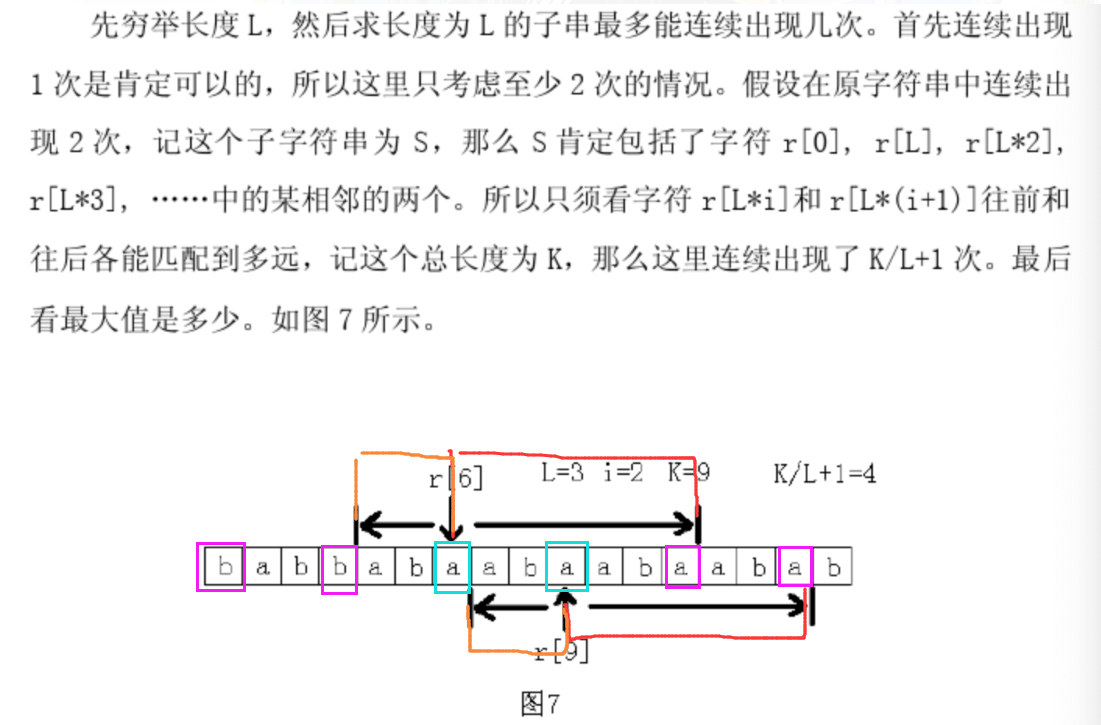
\includegraphics[width=10cm]{images/repeats.png}
\end{figure}
\par \noindent 具体的枚举长度 $L=2$ 时,上图紫色和青色是关键的的位置,考虑两个青色的(相邻)关键点,红色部分是往后扩展的长度,橘色部分是往前扩展的长度(正反串的 $\text{lcp}(j, j+L)$ )然后加起来就是循环长度。

\begin{minted}{c++}
ans = max(ans, (lcp(j, j+i)+lcp(N-j+1,N-(j+i)+1)+i-1)/i);
\end{minted}
\subsubsection{其他}
\begin{itemize}
    \item 求某两个后缀的最长公共前缀:$suffix(j)$ 和 $suffix(k)$ 的最长公共前缀为:$min\{height[rank[j] + 1], height[rank[j] + 2], ... height[rank[k]]\}$;这是一个 RMQ 问题,可以用 ST 表$O(nlogn)$ 预处理,$O(1)$ 查询。
    \item 可重叠最长重复子串:子串一定是某个后缀的前缀;可重叠的子串则等价于求两个后缀的最长公共前缀,所以求 $height[]$ 数组的最大值即可。
    \item 不可重叠最长重复子串:首先在 $[1...max(height)]$ 区间二分答案 $k$,判断是否存在两个长度为 $k$ 的子串是相同且不重叠的。利用 $height$ 值对后缀分组,使得每组的 $height$ 值都不小于 $k$(如果不存在就单独分组)。有希望成为最长公共前缀不小于 k 的两个后缀一定在同一组。然
    后对于每组后缀,只须判断每个后缀的 $sa$ 值的最大值和最小值之差是否不小于 $k$。
    \item 可重叠并出现 $k$ 次的最长重复子串:同样先二分长度答案 $x$ 分成若干组,判断的是有没有一个组的后缀个数不小于 $k$. 如果存在则满足条件。
    \item 不相同的子串个数:因为子串一定是某个后缀的前缀,问题等价于求所有后缀之间不相同的前缀的个数,如果所有的后缀按照 $suffix(sa[i])$ (排名)的顺序计算,对于新加入的后缀 $suffix(sa[k])$,将贡献 $n - sa[k] + 1 - height[k]$ 个不同的子串,累加即可。
    \item 最长回文子串:将整个字符串反过来接在原字符的后面,中间用一个特殊的字符隔开,求新字符串某两个后缀的最长公共前缀即可。
    \item 连续重复子串:(定义:字符串 $L$ 由某个字符串 $S$ 重复 $r$ 次得到,则 $L$ 称为连续重复子串)
    \item 求 $r$ 的最大值:枚举字符串 $S$ 的长度 $k$,然后判断是否满足。判断时先看 $L$ 的长度能否被 $k$ 整除,再看 $suffix(1)$ 和 $suffix(k+1)$ 的最长公共前缀是否等于 $n-k$,如果是则合法。
    \item 重复次数最多的连续重复子串:首先预处理 LCP;枚举重复部分的长度 $l$,然后枚举每一个起始位置$i$。如果重复部分出现大于等于 2 次,那么一定会有 $s[0], s[l], s[2*l]...s[k*l]$ 其中两个连续出现在重复组成的串中。所以对于确定的长度,$O(1)$ 查询 $s[i]$ 和 $s[i+l]$ 的公共前缀,然后向前向后匹配,重复串长度即为 $lcp(i, i + l) + (l - k \% l)$,然后再检查一下起点 $t=i-l+k\%l$ 是否溢出,以及 $lcp(t, t+l)$ 的长度是否大于 $k$ 即可更新答案。时间复杂度为 $O(nlogn)$.
    \item $A,B$ 的最长公共子串:首先把 $B$ 连接到 $A$ 的末尾,两者中间用一个没出现过的字符(如\$隔开),然后求新串的后缀数组、height 数组等。然后遍历 height 数组,当 $suffix(sa[i])$ 和 $suffix(sa[i-1])$ 不是同一个字符串中的两个后缀时,最大的$height[i]$就满足条件。判断 $suffix(sa[i])$ 和 $suffix(sa[i-1])$ 是否为同一个字符串中的两个后缀,只需判断下标的位置即可。
    \item $A,B$ 的长度不小于 $k$ 的公共子串个数(可以相同):思路是计算 A, B 的所有后缀之间的 lcp 的长度,统计 $lcp \ge k$ 的答案。首先把 $B$ 连接到 $A$ 的末尾,两者中间用一个没出现过的字符(如\$隔开),计算 height 后按 height 值大于等于 $k$ 分组。然后将后缀扫描一遍,遇到一个 B 的后缀就统计与前面的 A 的后缀能产生多少个长度不小于 $k$ 的公共子串。A 的后缀可以用单调栈维护;然后将 A 用相同的办法统计一次。
    \item 给定 $n$ 个字符串,求出现在不小于 $k$ 个字符串中的最长子串:将 $n$ 个字符串连接,中间用没出现过的字符隔开,求后缀数组。然后二分长度 $l$ 并利用 $height$ 数组分组,判断每组的后缀是否出现在不小于 $k$ 个原串中。
    \item 给定 $n$ 个字符串,求在每个字符串中至少出现两次且不重叠的最长子串:和上面一样,判断的时候,要看是否有一组后缀在每个原来的字符串中至少出现两次,并且在每个原来的字符串中,后缀的起始位置的最大值与最小值之差是否不小于当前答案(判断能否做到不重叠,如果题目中没有不重叠的要求,那么不用做此判断).
    \item 给定 $n$ 个字符串,求出现或反转后出现在每个字符串中的最长子串:将每个字符串反转后的结果也拼到总串中,求后缀数组。判断的时候,要看是否有一组后缀在每个原来的字符串或反转后的字符串中出现.
\end{itemize}

\clearpage